
\chapter{基于一维卷积神经网络的三维人体姿态序列估计}
\echapter{Preface}


\section{基于深度学习的三维人体姿态估计}


在人们生活中的各个场景中,RGB摄像头是最为普遍且性价比较高的摄像头。尽管在三维重建等计算机视觉任务中,能够提供深度信息的RGB-D摄像头得到了一定的认可,但由于其所使用的环境严格受限且价格昂贵等因素,对于针对日常生活场景的人体姿态估计任务不具备普遍的意义。同时,在更多的场景下,针对运动中的人体,通常只具备用一个固定位姿的单目RGB摄像机拍摄的条件。而此时所采集的人体运动图像及视频,无法记录和传达各个物体以及人体的深度信息。人眼所观察到的深度信息主要来源于以下三条规律:

\begin{enumerate}
    \item “近大远小”的眼球成像规则;
    \item 空间语义信息,如遮挡、熟悉动作的普遍位移方向等;
    \item 眼睛聚焦到目标物体时,睫状肌放松和紧张的感受以及眼压的大小。
\end{enumerate}

而上述规律对神经网络来说,学习难度极高。第一条规则受于目标人物的骨骼长度与学习样本的差异,以及视角的影响,第二条规则依赖于足够多样性的数据和网络自身的鲁棒性,第三条规则则不能够被现有的传感器模拟。而由于多个三维人体关节点坐标都可以投影到相同的一个二维姿态,缺失了深度信息的三维姿态恢复具有着理论上无法消除的歧义性。综上所述,对单目RGB图像及视频中的人体姿态三维关节点坐标的估计,尤其是全局三维坐标的估计具有极大的挑战。近几年解决三维人体姿态估计的工作主要分为本文第一章中已有所介绍的两种思路,端到端式和两步式。由于二维姿态估计的发展在深度学习和良好的数据集的推动下已经较为成熟,两步式方案普遍具有着更高的效率和更好的表现。

同时,虽然用相机获得直接的深度信息,或进行多目相机的多视角记录具有较小的现实意义。同时,由于二维图像提升至三维坐标本身具有歧义性\textsuperscript{\cite{p12}},即多个三维姿态可以映射到相同的二维关键点。而视频上下文中人体运动的合理性及连贯性约束,使得帧序列之间的时序信息提取对消除歧义性有着极大的价值,故而在针对视频序列进行人体姿态估计时,可以采取时序模型对相邻帧之间的时间信息进行提取。之前的工作主要通过使用循环神经网络及长短期记忆网络进行时序信息处理。如Hossain等在2018年提出的Lee等在2018年提出的Propagating LSTM等。

\section{模型与方法}
在利用第三章种搭建的二维人体姿态估计网络提取出图像中的人体二维关节点坐标后,本章网络模型采取经典的两步提升操作,利用VideoPose3D三维人体姿态估计模型\textsuperscript{\cite{p26}}进一步估计关节点的三维坐标。

本文采用一种基于二维关键点轨迹的一维空洞卷积处理连续帧序列中的时序信息,预测视频中的三维姿态。本文采用一个具有残余连接的完全卷积结构,它将一系列二维姿态作为输入,并通过时间维度上的卷积对它们进行转换。并利用空洞卷积,来扩展估计每一帧姿态时的时序信息的感受野,处理更大范围的上下文信息。

与依赖于循环神经网络的方法相比,它在一定的计算复杂度和参数数量具有更高的准确性、简单性和效率。首先,卷积模型支持批处理和时间维度上的并行,而循环神经网络不能随着时间的推移而并行。其次,无论序列长度如何,卷积网络的输出和输入之间的梯度路径都有固定的长度,这缓解了影响循环神经网络的消失和爆炸梯度。除此之外,卷积结构还可以对平级的时序信息有更为精确的感知,更适用于在三维姿态估计任务。

本文的网络结构如图\ref{fig:f23}所示,卷积层为绿色的模块。网络的输入为视频连续的243帧中人体J(J=17)个关节点的二维坐标(x,y),即2*J个通道的数据,送入卷积核大小为W(W=3)且具有c(c=1024)个输出通道的时序卷积模型。接着连接B(B=4)个带有跳跃连接的残差块,每个残差块由一个空洞系数为D=WB的一维卷积层和一个卷积核大小为1的卷积层构成。除了最后一层卷积层外,每个卷积层后接有批标准化(BN, Batch Normalization),ReLU线性修正单元和因子为p(p=0.25)Dropout正则化操作。

\begin{figure}[h]
	\centering
	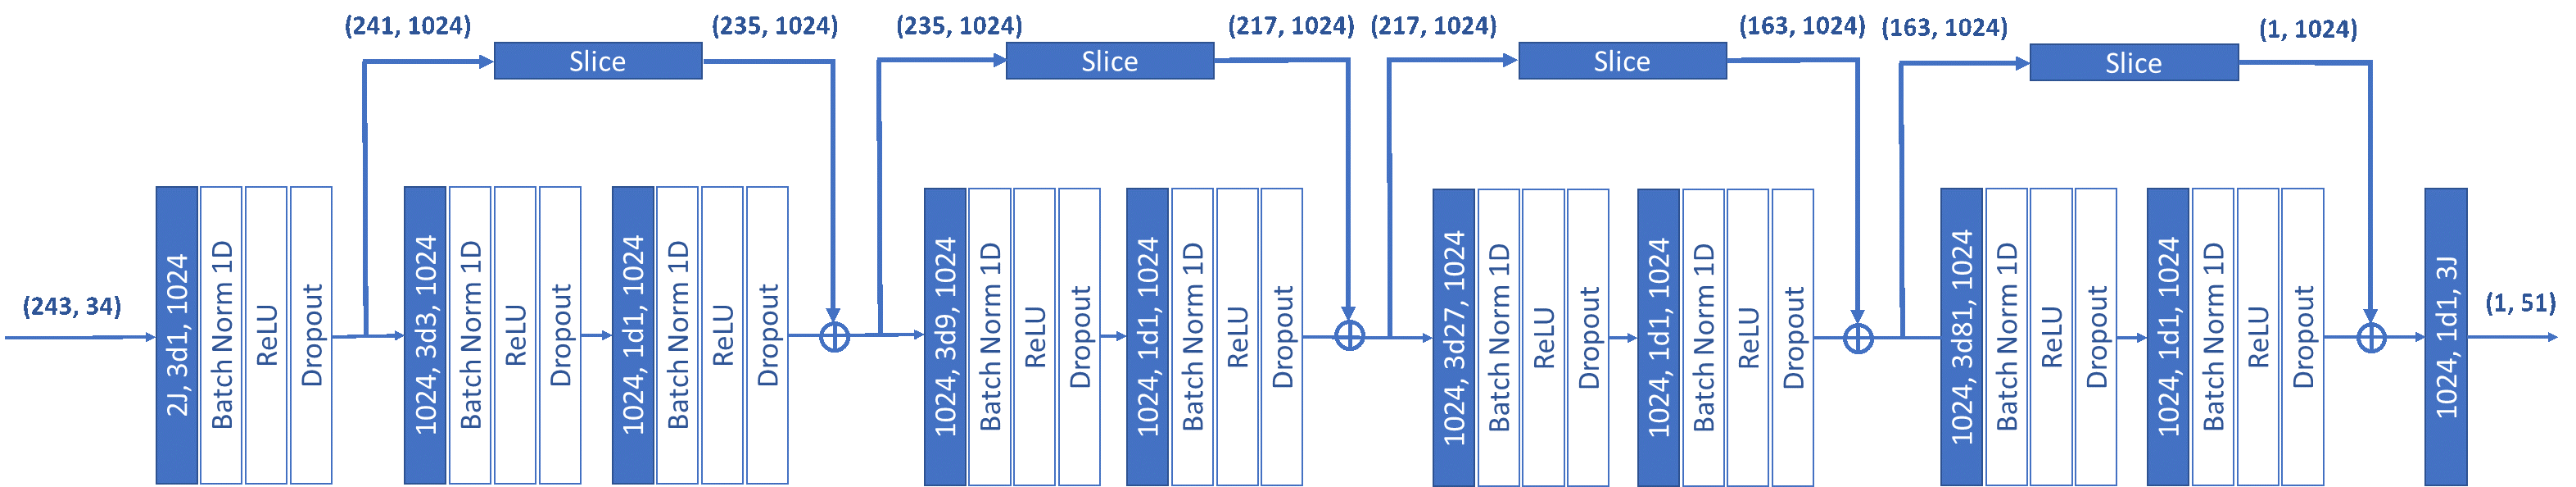
\includegraphics[scale=0.4]{figures/23.png}
	\caption{三维人体姿态估计模型网络结构}
	\label{fig:f23}
\end{figure}

在如上模型中每个残差块的感受野以W进行指数增加时,保证了参数的数量仅为线性增加。卷积核的大小W及空洞系数D使得感受野以树状覆盖所有的输入帧。最终网络输出所有帧的人体三维姿态。

\begin{figure}[h]
	\centering
	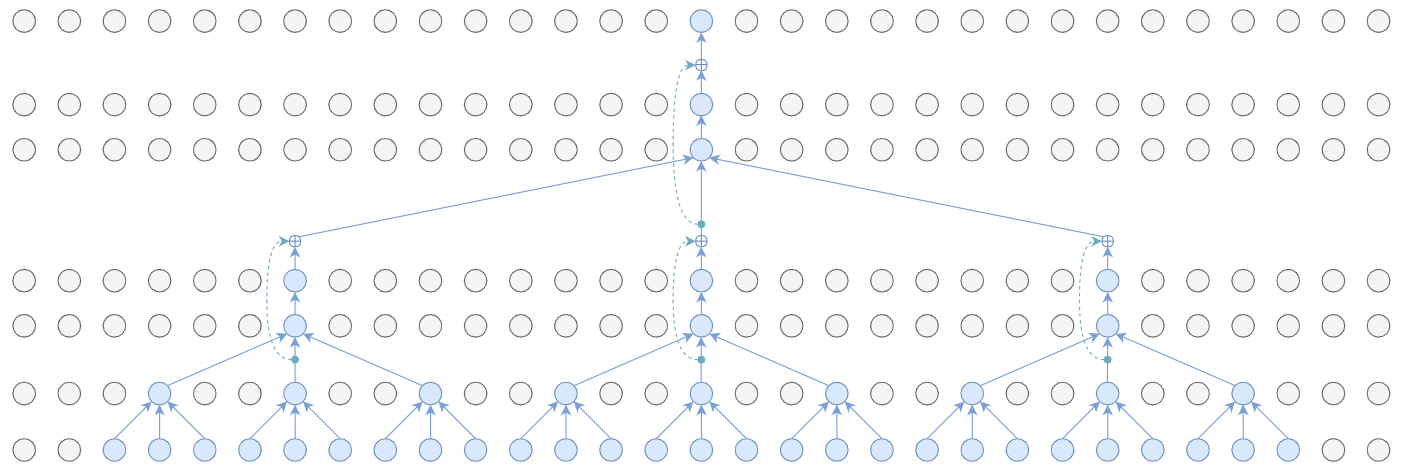
\includegraphics[scale=0.4]{figures/24.png}
	\caption{树状网络模型(W=3,B=3)\textsuperscript{\cite{p26}}}
	\label{fig:f24}
\end{figure}


\section{数据及实验}
\subsection{三维人体姿态数据集}{}
Human3.6M数据集具有360万个三维人体姿势和相应的图像,共11位实验者包括6位男性和5位女性\textsuperscript{\cite{p16}},共有17个动作场景,诸如讨论、吃饭、运动、问候等动作。用4个严格校准的相机录制高分辨率的50Hz视频。并用高速运动动作捕捉系统提供准确的关节点三维位置,像素级的24个人体部位信息。同时严格控制背景元素,提供精准的人体位置边框。

HumanEva-I数据集包含用三个60赫兹的摄像机记录的经过校准的视频序列(4个灰度视频和3个RGB视频),与从运动捕捉系统获得的三维身体姿态同步。该数据库包含4名受试者执行6种常见动作(如散步、慢跑、打手势等)\textsuperscript{\cite{p15}}。给出了二维和三维姿态中计算误差的误差度量。该数据集包含训练、验证和测试集。本文采用15个关节点信息进行训练和测试。

PI-INF-3DHP 数据集,由 Max Planck Institute for Informatics 制作,是一个新发布的三维人体姿势数据集,包含 6 个7 个动作(背景为绿屏 (GS) 和无绿屏 (NoGS)),由动 (MoCap System)和 14 个 RGB 相机和 2 名受试者在室外的野外设置中执行动作。

由卡内基梅隆大学(CMU, Carnegie Mellon University)制作。使用了480个VGA摄像头,具有640 x 480的分辨率,视频帧率为25 fps,并使用了与其同步的31个HD摄像头,具有1920 x 1080分辨率,帧率为30 fps,在它们之间同步使用硬件时钟。同时,还使用了10个KinectⅡ传感器和5个DLP投影仪。采集了时长共5.5小时的65个视频序列,包含了150万个三维人体骨架信息。

在本文的工作中,选取Human3.6m数据集中的17个关节点信息,在(S1、S5、S6、S7、S8) 5个子集上进行训练,并用(S9、S11)2个子集作为测试集。

\subsection{实验结果}{}
本文使用评价指标为关节点平均坐标误差MPJPE (Mean Peer Joint Position Error),估计出的坐标与真实关节点坐标之间的欧氏距离。

本文采用Adam优化器,设置learning rate=0.001, decay=0.95,同时batch size=1024对Human3.6m数据集进行80 epoches的训练,训练及测试结果如下所示。

\begin{figure}[h]
	\centering
	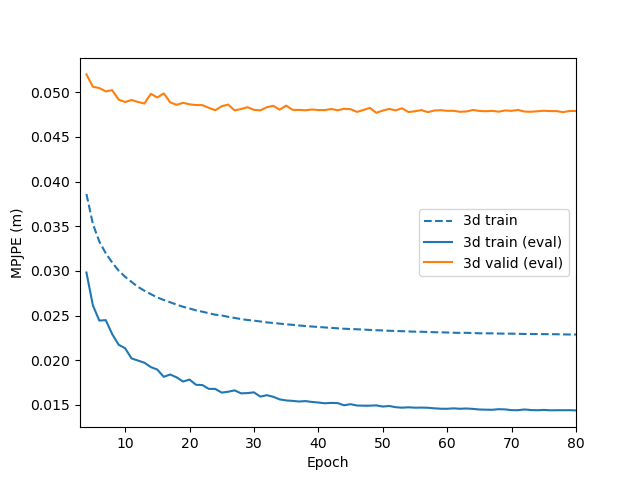
\includegraphics[scale=1]{figures/25.png}
	\caption{三维人体姿态估计模型MPJPE-Epoch曲线}
	\label{fig:f25}
\end{figure}


\begin{table}[h]
    \caption{\label{tab:t3}二维人体姿态估计模型测试结果}
    \centering
    \begin{tabular}{c c c c c c c c c c c c c c c c c c}
        \toprule
		Methods  & Dir.   & Disc. & Eat   & Greet  & Phone  & Photo  & Pose  & Purch.  & Sit  & SitD.  & Smoke  & Wait  & WalkD.  & Walk  & WalkT.  & Avg   \\
        \midrule
        Pavlakos et al. CVPR’17\textsuperscript{\cite{p1}}     & 67.4  & 71.9  & 66.7  & 69.1  & 72.0  & 77.0  & 65.0  & 68.3  & 83.7  & 96.5  & 71.7  & 65.8  & 74.9  & 59.1  & 63.2  & 71.9  \\
		Tekin et al. ICCV’17\textsuperscript{\cite{p2}}        & 54.2  & 61.4  & 60.2  & 61.2  & 79.4  & 78.3  & 63.1  & 81.6  & 70.1  & 107.3 & 69.3  & 70.3  & 74.3  & 51.8  & 63.2  & 69.7  \\
		Martinez et al. ICCV’17\textsuperscript{\cite{p30}}    & 51.8  & 56.2  & 58.1  & 59.0  & 69.5  & 78.4  & 55.2  & 58.1  & 74.0  & 94.6  & 62.3  & 59.1  & 65.1  & 49.5  & 52.4  & 62.9  \\
		Sun et al. ICCV’17\textsuperscript{\cite{p3}}          & 52.8  & 54.8  & 54.2  & 54.3  & 61.8  & 67.2  & 53.1  & 53.6  & 71.7  & 86.7  & 61.5  & 53.4  & 61.6  & 47.1  & 53.4  & 59.1  \\
		Fang et al. AAAI’18\textsuperscript{\cite{p4}}         & 50.1  & 54.3  & 57.0  & 57.1  & 66.6  & 73.3  & 53.4  & 55.7  & 72.8  & 88.6  & 60.3  & 57.7  & 62.7  & 47.5  & 50.6  & 60.4  \\
		Pavlakos et al. CVPR’\textsuperscript{\cite{p5}}       & 48.5  & 54.4  & 54.4  & 52.0  & 59.4  & 65.3  & 49.9  & 52.9  & 65.8  & 71.1  & 56.6  & 52.9  & 60.9  & 44.7  & 47.8  & 56.2  \\
		Yang et al. CVPR’18\textsuperscript{\cite{p6}}         & 51.5  & 58.9  & 50.4  & 57.0  & 62.1  & 65.4  & 49.8  & 52.7  & 69.2  & 85.2  & 57.4  & 58.4  & 43.6  & 60.1  & 47.7  & 58.6  \\
		Luvizon et al. CVPR’18\textsuperscript{\cite{p7}}      & 49.2  & 51.6  & 47.6  & 50.5  & 51.8  & 60.3  & 48.5  & 51.7  & 61.5  & 70.9  & 53.7  & 48.9  & 57.9  & 44.4  & 48.9  & 53.2  \\
		Hossain  ECCV’18\textsuperscript{\cite{p8}}            & 48.4  & 50.7  & 57.2  & 55.2  & 63.1  & 72.6  & 53.0  & 51.7  & 66.1  & 80.9  & 59.0  & 57.3  & 62.4  & 46.6  & 49.6  & 58.3  \\
        Lee et al.ECCV’18\textsuperscript{\cite{p11}}  	       & 40.2  & 49.2  & 47.8  & 52.6  & 50.1  & 75.0  & 50.2  & 43.0  & 55.8  & 73.9  & 54.1  & 55.6  & 58.2  & 43.3  & 43.3  & 52.8 \\
		Ours                                                   & 45.0  & 46.6  & 42.2  & 45.6  & 48.6  & 56.0  & 44.1  & 43.7  & 57.2  & 65.0  & 47.2  & 43.8  & 49.2  & 33.0  & 33.8  & 46.7  \\
		\bottomrule
    \end{tabular}
\end{table}


在针对Human3.6m数据集的姿态估计中,本文的方法可以流畅准确地还原出人体的三维动作,以该视频为例,本文的工作的输出结果与真实标注的差异如图\ref{fig:f26}所示。可见估计结果中的三维姿态强依赖于二维关节点坐标,基本保证了三维姿态到相机坐标系的重投影与二维姿态一致。

\begin{figure}[h]
	\centering
	\includegraphics[scale=0.2]{figures/26.png}
	\caption{三维人体姿态估计结果对比真实标注(数据为Photo.54138969)}
	\label{fig:f26}
\end{figure}













